\section{Algorithms}

\subsection{Finding frequent episodes: high-level algorithm}

\begin{algorithm}

\caption{High-level algorithm for finding frequent episodes. \\
Input: A set $ \Sigma $ of event types, an event sequence $ s $ over $ \Sigma $, a window width \emph{win}, and a frequency threshold \emph{min\_fr}. \\
Output: The collection of episodes that are frequent in the sequence in terms of the input parameters.
}

\begin{algorithmic}[1]

\State $ \mathcal{C} \gets \{ \alpha \mid | \alpha | = 1 \} $
\State $ l \gets 1 $
\While{$ \mathcal{C}_l \neq \emptyset $}
    \LineComment{Database pass (algorithms \ref{alg:rec-par-fwi}, \ref{alg:rec-ser-fwi}, ...)}
    \State compute $ \mathcal{F}_l \gets \{ \alpha \in \mathcal{C}_l | fr(\alpha, s, \text{win}) \geq \text{min\_fr} \} $
    \State $ l \gets l + 1 $
    \LineComment{Candidate generation (algorithm \ref{alg:cand-gen})}
    \State compute $ C_l = \{ \alpha \mid | \alpha | = l \wedge \forall \beta \mid \beta \subset \alpha : \beta \text{ is frequent} \} $
\EndWhile
\State output all $ \mathcal{F}_i $

\end{algorithmic}

\label{alg:episodes-top-level}
\end{algorithm}

% TODO Read this future me, probably needs improvement. Also why question marks??

Algorithm~\ref{alg:episodes-top-level} describes the high-level procedure to find all frequent episodes of a certain class (parallel or serial) that are frequent in an event sequence $ s $, given window width \emph{win} and frequency threshold \emph{min\_fr}. It is a breadth-first algorithm, that is, all frequent episodes of size $ l $ are computed before those of size $ l + 1 $.

The first set of candidates $ \mathcal{C}_1 $ consists of all episodes of size $ 1 $. After constructing $ \mathcal{C}_1 $ a loop is entered where for each $ l $, it is determined which episodes are frequent ($ \mathcal{F}_1 $), by a pass over the sequence, and subsequently, based on those, candidates of size $ 2 $ are generated. The loop continues with ever-increasing episode size $ l $, and stops when no more candidates were generated. Then all frequent episodes have been found.

The following subsections will cover all of the subalgorithms.

\subsection{Candidate generation}
\label{sec:cand-gen}

\begin{algorithm}

\caption{Generating candidate parallel episodes of size $ l + 1 $ from frequent parallel episodes of size $ l $. \\
Input: A sorted array $ \mathcal{F}_l $ of frequent parallel episodes of size $ l $. \\
Output: A sorted array of candidate parallel episodes of size $ l + 1 $.
}

\begin{algorithmic}[1]

\State $ \mathcal{C}_{l + 1} \gets \emptyset $
\State $ k \gets 0 $
\If{$ l = 1 $}
    \For{$ h \gets 1 $ to $ | \mathcal{F}_l | $} $ \mathcal{F}_l \text{.block\_start}[h] \gets 1 $ \EndFor
\EndIf
\For{$ i \gets 1 $ to $ | \mathcal{F}_l | $}
    \State $ \text{current\_block\_start} \gets k + 1 $
    \For{$ j \gets i $; $ \mathcal{F}_l \text{.block\_start}[j] = \mathcal{F}_l \text{.block\_start}[i] $; $ j \gets j + 1 $}
    \label{alglin:cand-gen:j-loop}
        \LineComment{$ \mathcal{F}_l[i] $ and $ \mathcal{F}_l[j] $ have $ l - 1 $ first event types in common, build a potential candidate $ \alpha $ as their combination.}
        \For{$ x \gets 1 $ to $ l $} $ \alpha[x] \gets \mathcal{F}_l[i][x] $
        \EndFor
        \State $ \alpha[l + 1] \gets \mathcal{F}_l[j][l] $
        \LineComment{Build and test subepisodes $ \beta $ that do not contain $ \alpha[y] $}
        \For{$ y \gets 1 $ to $ l - 1 $}
            \For{$ x \gets 1 $ to $ y - 1 $} $ \beta[x] \gets \alpha[y] $
            \EndFor
            \For{$ x \gets y $ to $ l $} $ \beta[x] \gets \alpha[x + 1] $
            \EndFor
            \If{$ \beta $ is not in $ \mathcal{F}_l} $ continue with the next $ j $ at line~\ref{alglin:cand-gen:j-loop}
            \EndIf
        \EndFor
        \LineComment{All subepisodes are in $ \mathcal{F}_l $, store $ \alpha $ as candidate}
        \State $ k \gets k + 1 $
        \State $ \mathcal{C}_{l + 1}[k] \gets \alpha $
        \State $ \mathcal{C}_{l + 1} \text{.block\_start}[k] \gets \text{current\_block\_start} $
    \EndFor
\EndFor
\State output $ \mathcal{C}_{l + 1} $

\end{algorithmic}

\label{alg:cand-gen}
\end{algorithm}

Algorithm~\ref{alg:cand-gen} generates candidates of size $ l + 1 $ from a collection of frequent parallel episodes of size $ l $. It can be easily modified to generate serial episodes, as we'll show later in this subsection. Thanks to the monotonic property of the frequency measures we implement, some candidates can be immediately proven infrequent. More specifically, if there exists an infrequent subepisode $ \beta $ of candidate $ \alpha $, then $ \alpha $ is not frequent.
Conveniently, all frequent subepisodes of size $ l $ are already given as input to the algorithm. So when the algorithm constructs a candidate of size $ l + 1 $, all of its subepisodes of size $ l $ are checked to be frequent by testing whether they are in the input collection $ \mathcal{F}_l $. If one of the subepisodes is not in $ \mathcal{F}_l $, then it is infrequent and, consequently, the potential candidate cannot be frequent either.
Smaller subepisodes do not need to be checked anymore, because any $ l $-sized episodes that have turned out to be frequent are already known to have frequent subepisodes.

Parallel episodes are constructed such that the elements in their arrays are sorted according to event type. In this way, a parallel episode has a unique array representation.

Potential candidates of size $ l + 1 $ are generated by combining frequent episodes of size $ l $ which share a prefix of $ l - 1 $ elements. In other words, a candidate is generated from episodes $ x $ and $ y $ which can only differ in their last element. The newly constructed candidate shares these $ l - 1 $ as well, and is then followed by the last elements of both $ x $ and $ y $. This method of candidate generation is similar to the way in which candidate itemsets are generated in the Apriori [cite] algorithm. Figure~\ref{fig:parallel-episode-lattice} shows visually how larger candidates build upon smaller episodes.

% TODO illustrate two episodes being combined with each other

\begin{figure}
\centering

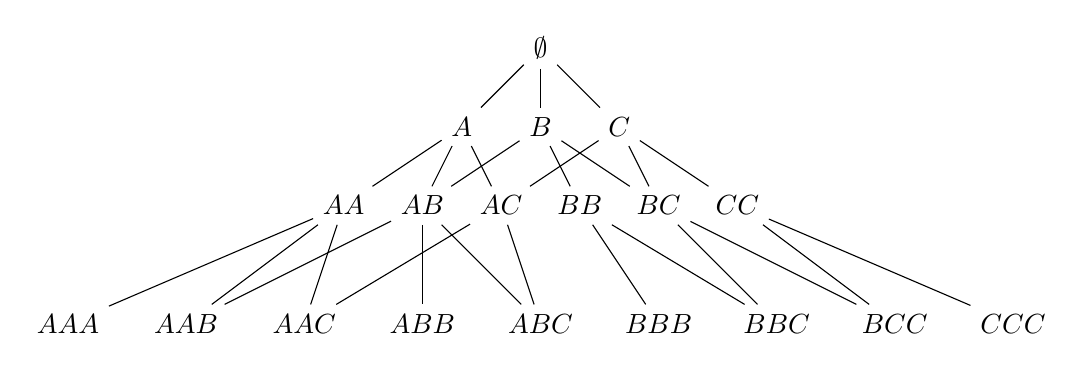
\begin{tikzpicture}

\node (e) at (0,0) {$ \emptyset $};
\node (A) at (-1,-1) {$ A $};
\node (B) at (0,-1) {$ B $};
\node (C) at (1, -1) {$ C $};

\node (AA) at (-2.5,-2) {$ AA $};
\node (AB) at (-1.5,-2) {$ AB $};
\node (AC) at (-0.5,-2) {$ AC $};
\node (BB) at (0.5,-2) {$ BB $};
\node (BC) at (1.5,-2) {$ BC $};
\node (CC) at (2.5,-2) {$ CC $};

\node (AAA) at (-6,-3.5) {$ AAA $};
\node (AAB) at (-4.5,-3.5) {$ AAB $};
\node (AAC) at (-3,-3.5) {$ AAC $};
\node (ABB) at (-1.5,-3.5) {$ ABB $};
\node (ABC) at (0,-3.5) {$ ABC $};
\node (BBB) at (1.5,-3.5) {$ BBB $};
\node (BBC) at (3,-3.5) {$ BBC $};
\node (BCC) at (4.5,-3.5) {$ BCC $};
\node (CCC) at (6,-3.5) {$ CCC $};

\draw (e) -- (A);
\draw (e) -- (B);
\draw (e) -- (C);

\draw (A) -- (AA);
\draw (A) -- (AB);
\draw (B) -- (AB);
\draw (A) -- (AC);
\draw (C) -- (AC);
\draw (B) -- (BB);
\draw (B) -- (BC);
\draw (C) -- (BC);
\draw (C) -- (CC);

\draw (AA) -- (AAA);
\draw (AA) -- (AAB);
\draw (AB) -- (AAB);
\draw (AB) -- (ABB);
\draw (AA) -- (AAC);
\draw (AC) -- (AAC);
\draw (AB) -- (ABC);
\draw (AC) -- (ABC);
\draw (BB) -- (BBB);
\draw (BB) -- (BBC);
\draw (BC) -- (BBC);
\draw (BC) -- (BCC);
\draw (CC) -- (BCC);
\draw (CC) -- (CCC);

\end{tikzpicture}

\caption{The lattice of parallel episode construction for $ \Sigma = \{ A, B, C \} $ up to size 3.}

\label{fig:parallel-episode-lattice}
\end{figure}

The algorithm assumes that the input array of frequent $ l $-sized episodes $ \mathcal{F}_l $ is sorted lexicographically. That is, the episodes are primarily sorted by the first event type in the array, secondarily by the second element, and so on. The algorithm constructs new episodes in such a way that the output is ordered in the same manner, and since the ordering is preserved when filtering episodes, the input never needs to be sorted before running the candidate generation algorithm.

As mentioned previously, a potential candidate is generated from two episodes that share an $ (l - 1) $-prefix. And with the episodes being ordered as described, all of the episodes that share a prefix in their array representation are grouped together. As a result, episodes can be grouped into blocks where all of the episodes in a block share the first $ l - 1 $ elements. Figure~\ref{fig:blocks} illustrates this block structure.



\begin{figure}
\centering

\begin{tikzpicture}[accolade/.style={decorate,decoration={brace,amplitude=10pt}}]

\newcommand\blockspicvalue[2]{
    \ifcase#2
        \ifcase#1 A
            \or A
            \or B
        \fi
        \or \ifcase#1 A
            \or A
            \or C
        \fi
        \or \ifcase#1 A
            \or C
            \or C
        \fi
        \or \ifcase#1 A
            \or C
            \or D
        \fi
        \or B
        \or \ifcase#1 B
            \or B
            \or C
        \fi
        \or \ifcase#1 B
            \or B
            \or D
        \fi
        \or C
    \fi
}

\foreach \x in {0,...,2}
\foreach \y in {0,...,7}
{
    \node (n\x\y) [draw,minimum size=1cm] at (\x,-\y*1.1) {$ \blockspicvalue{\x}{\y} $};
}

\draw[accolade]([yshift=2pt]n00.north west) -- ([yshift=2pt]n10.north east) node [midway,above=12pt] {episodes with shared 2-prefix form a block};

\draw [accolade] ([xshift=2pt]n20.north east) -- ([xshift=2pt]n21.south east) node [midway,right=12pt] {block};
\draw [accolade] ([xshift=2pt]n22.north east) -- ([xshift=2pt]n23.south east) node [midway,right=12pt] {block};
\draw [accolade] ([xshift=2pt]n24.north east) -- ([xshift=2pt]n26.south east) node [midway,right=12pt] {block};
\draw [decorate,decoration={brace,amplitude=5pt}] ([xshift=2pt]n27.north east) -- ([xshift=2pt]n27.south east) node [midway,right=12pt] {block};

\end{tikzpicture}

\caption{Blocks in candidate generation algorithm with parallel episodes of size 3.}

\label{fig:blocks}
\end{figure}

This block structure is represented as follows.
Each episode $ \alpha $ includes a value \emph{block\_start}, which is the array index of the first episode in the block which contains $ \alpha $, so it points ``back'' to the beginning of the block. (The first episode in each block points to itself.) In this way, it can be easily tested whether two episodes belong to the same block.

The algorithm constructs this block structure while generating candidates of size $ l + 1 $, but it also uses the blocks of the $ l $-sized episodes given as input. So it is important that they are preserved and maintained in between different runs of algorithm~\ref{alg:cand-gen}. Section~\ref{sec:maintain-blocks} goes into more detail about this.

Constructing all $ (| \alpha | - 1) $-sized subepisodes of an episode $ \alpha $ is straightforward. For each subepisode, one node from $ \alpha $'s graph is left out, until all nodes have been left out. For serial episodes, the edges of the subepisode are constructed such that the order of the toplogical sort is preserved. (If we consider the strict form of a serial candidate, a subepisode can be obtained by leaving one node $ v $ and all edges that contain $ v $.) For the array representation of both classes of episodes, this means that one element of the array is left out.

% TODO illustrate construction of subepisodes

\subsection{Recognizing parallel episodes with fixed windows}

\begin{algorithm}

\caption{Recognizing parallel episodes using the fixed-window frequency measure. \\
Input: A collection $ \mathcal{C} $ of parallel episodes, an event sequence $ \boldsymbol{s} = (s, T_s, T_e) $, a window width \textit{win}, and a frequency threshold \textit{min\_fr}. \\
Output: The episodes of $ \mathcal{C} $ that are frequent in $ \boldsymbol{s} $ with respect to \textit{win} and \textit{min\_fr}.
}

\begin{algorithmic}[1]

\LineComment{Initialization}
\ForAll{$ \alpha $ in $ \mathcal{C} $}
    \ForAll{$ A $ in $ \alpha $}
        \State $ A \text{.count} \gets 0 $
        \For{$ i \gets 1 $ to $ | \alpha | $} $ \text{contains}(A, i) \gets \emptyset $ \EndFor
    \EndFor
\EndFor

\ForAll{$ \alpha $ in $ \mathcal{C} $}
    \ForAll{$ A $ in $ \alpha $}
        \State $ a \gets $ number of elements of type $ A $ in $ \alpha $
        \State $ \text{contains}(A, a) \gets \text{contains}(A, a) \cup \{ \alpha \} $
    \EndFor
    \State $ \alpha \text{.event\_count} \gets 0 $
    \State $ \alpha \text{.freq\_count} \gets 0 $
\EndFor

\LineComment{Recognition}
\For{$ \text{start} \gets T_s - \text{win} + 1 $ to $ T_e $}
    \LineComment{Bring new events to the window}
    \ForAll{events $ (A, t) $ in $ s $ such that $ t = \text{start} + \text{win} - 1 $} \label{alglin:rec-par-fwi:new-events}
        \State $ A \text{.event\_count} \gets A \text{.event\_count} + 1 $
        \ForAll{$ \alpha \in \text{contains}(A, A \text{.count}) $}
            \State $ \alpha \text{.event\_count} \gets \alpha \text{.event\_count} + A \text{.count} $
            \If{$ \alpha \text{.event\_count} = | \alpha | $} $ \alpha \text{.in\_window} \gets \text{start} $
            \EndIf
        \EndFor
    \EndFor
    \LineComment{Drop out old events from the window}
    \ForAll{events $ (A, t) $ in $ s $ such that $ t = \text{start} - 1 $} \label{alglin:rec-par-fwi:old-events}
        \ForAll{$ \alpha \in \text{contains}(A, A \text{.count}) $}
            \If{$ \alpha \text{.event\_count} = | \alpha | $}
                \State $ \alpha \text{.freq\_count} \gets \alpha \text{.freq\_count} - \alpha \text{.in\_window} + \text{start} $
            \EndIf
            \State $ \alpha \text{.event\_count} \gets \alpha \text{.event\_count} - A \text{.count} $
        \EndFor
        \State $ A \text{.event\_count} \gets A \text{.event\_count} - 1 $
    \EndFor
\EndFor
\LineComment{Output}
\ForAll{episodes $ \alpha $ in $ \mathcal{C} $}
    \If{$ \alpha \text{.freq\_count} / (T_e - T_s + \text{win} - 1) \geq \text{min\_fr} $} output $ \alpha $
    \EndIf
\EndFor

\end{algorithmic}

\label{alg:rec-par-fwi}
\end{algorithm}

Algorithm~\ref{alg:rec-par-fwi} recognizes parallel episodes in an event sequence. As stated before, parallel episodes impose no order on the occurrence of events in the window. Therefore, to recognize an episode in the sequence, it suffices to know that there are enough events of each type currently in the window. More formally, an episode $ \alpha $ occurs in a window if for each event type $ A $, the window contains at least as many events of type $ A $ as there are nodes of type $ A $ in $ \alpha $'s graph. The algorithm makes one pass over the sequence.

Recognition is accomplished as follows. For each event type $ A $, a counter $ A \text{.count} $ is maintained. This counter denotes how many events of type $ A $ are currently in the window. When a new event of type $ A $ enters the window (line~\ref{alglin:rec-par-fwi:new-events} and further), this counter is increased by $ 1 $. Then, for all episodes $ \alpha $ containing $ A \text{.count} $ nodes of type $ A $, a per-episode counter $ \alpha \text{.event\_count} $ is increased by $ A \text{.count} $, indicating that there are currently enough events of type $ A $ in the window to satisfy an occurrence. If this is the case for all event types in $ \alpha $, then $ \alpha \text{.event\_count} = | \alpha | $, and so the window contains $ \alpha $. To mark the point in time at which the episode entered the sliding window, variable $ \alpha \text{.in\_window} $ gets set to \emph{start}.

When an event of type $ A $ leaves the window (line~\ref{alglin:rec-par-fwi:old-events} and further), for all episodes $ \alpha $ with $ A \text{.count} $ nodes of event type $ A $, if $ \alpha \text{.event\_count} = | \alpha | $, $ \alpha $ has been contained in a number of windows, but is now no longer. The episode was in $ (\text{start} - \alpha \text{.in\_window}) $ windows, and so $ \alpha \text{.freq\_count} $ gets updated accordingly. Next, $ A \text{.count} $ gets decreased by $ 1 $ to reflect the fact that an even of type $ A $ has left the sliding window.

\subsection{Recognizing serial episodes with fixed windows}

\begin{algorithm}

\caption{Recognizing serial episodes using the fixed-window frequency measure. \\
Input: A collection $ \mathcal{C} $ of serial episodes, an event sequence $ \boldsymbol{s} = (s, T_s, T_e) $, a window width \textit{win}, and a frequency threshold \textit{min\_fr}. \\
Ouptut: The episodes of $ \mathcal{C} $ that are frequent in $ \boldsymbol{s} $ with respect to \textit{win} and \textit{min\_fr}.
}

\begin{algorithmic}[1]

\LineComment{Initialization}
\ForAll{$ \alpha \in \mathcal{C} $}
    \For{$ i \leftarrow 1 $ to $ | \alpha | $}
        \State{$ \alpha \text{.initialized} \leftarrow \text{\textit{uninitialized}} $}
        \State{$ \text{waits}(\alpha[i]) \leftarrow 0 $}
    \EndFor
\EndFor

\ForAll{$ \alpha \in \mathcal{C} $}
    \State{$ \text{waits}(\alpha[1]) \leftarrow \text{waits}(\alpha[1]) \cup \left\{ \left( \alpha, 1 \right) \right\} $}
    \State{$ \alpha \text{.freq\_count} \leftarrow 0 $}
\EndFor

\For{$ t \leftarrow T_s - \text{win} $ to $ T_s - 1 $} $ \text{begins\_at}(t) \leftarrow \emptyset $
\EndFor

\LineComment{Recognition}
\For{$ \text{start} \leftarrow T_s - \text{win} + 1 $ to $ T_e $}
    \State{$ \text{begins\_at}(\text{start} + \text{win} - 1) \leftarrow \emptyset $}
    \State{$ \text{transitions} \leftarrow \emptyset $}
    \ForAll{events $ (A, t) $ in $ s $ such that $ t = \text{start} + \text{win} - 1 $}
        \ForAll{$ ( \alpha, j) \in \text{waits}(A) $}
            \If{$ j = | \alpha | \wedge \alpha \text{.initialized}[j] = \text{\textit{uninitialized}} $}
                \State{$ \alpha \text{.in\_window} \leftarrow \text{start} $}
            \EndIf
            \If{$ j = 1 $}
                \State{$ \text{transitions} \leftarrow \text{transitions} \cup \{ ( \alpha, 1, \text{start} + \text{win} - 1 ) \} $}
            \Else
                \State{$ \text{transitions} \leftarrow \text{transitions} \cup \{ \alpha, j, \alpha \text{.initialized} [j - 1] \} $}
                \State{$ \text{begins\_at}( \alpha \text{.initialized}[j - 1] ) \leftarrow $
                \State \hspace{\algorithmicindent} $ \text{begins\_at}( \alpha \text{.initialized}[j - 1] ) \setminus \{ ( \alpha, j - 1 ) \} $}
                \State{$ \alpha \text{.initialized} [j - 1] \leftarrow \text{\textit{uninitialized}} $}
                \State{$ \text{waits}(A) \leftarrow \text{waits}(A) \setminus \{ ( \alpha, j ) \} $}
            \EndIf
        \EndFor
    \EndFor
    \ForAll{$ ( \alpha, j, t ) \in \text{transitions} $}
        \State{$ \alpha \text{.initialized} [j] \leftarrow t $} \label{alglin:rec-ser-fwi:transition-begin}
        \State{$ \text{begins\_at}(t) \leftarrow \text{begins\_at}(t) \cup \{ ( \alpha, j ) \} $}
        \If{$ j < | \alpha | $}
            \State{$ \text{waits}(\alpha [j + 1]) \leftarrow \text{waits}(\alpha [j + 1]) \cup \{ (\alpha, j + 1) \} $} \label{alglin:rec-ser-fwi:transition-end}
        \EndIf
    \EndFor
    \ForAll{$ (\alpha, l) \in \text{begins\_at}(\text{start} - 1) $} \label{alglin:rec-ser-fwi:cleanup-for}
        \If{$ l = | \alpha | $} \label{alglin:rec-ser-fwi:cleanup-iteration-begin}
            \State{$ \alpha \text{.freq\_count} \leftarrow \alpha \text{.freq\_count} - \alpha \text{.in\_window} + \text{start} $}
        \Else
            \State{$ \text{waits}(\alpha [l + 1]) \leftarrow \text{waits}(\alpha [l + 1]) \setminus \{ ( \alpha, l + 1 ) \} $}
        \EndIf
        \State{$ \alpha \text{.initialized}[l] \leftarrow 0 $} \label{alglin:rec-ser-fwi:cleanup-iteration-end}
    \EndFor
\EndFor
\ForAll{episodes $ \alpha $ in $ \mathcal{C} $}
    \If{$ \alpha \text{.freq\_count} / T_e - T_s + \text{win} - 1 \geq \text{min\_fr} $}
        \State{output $ \alpha $}
    \EndIf
\EndFor

\end{algorithmic}

\label{alg:rec-ser-fwi}
\end{algorithm}

Algorithm~\ref{alg:rec-ser-fwi} is for recognizing serial episodes in a sequence. By the definition of serial episodes, all nodes must appear in the sequence in a strict order. Serial episodes are therefore recognized using automata, instances of which advance as events are encountered. The algorithm iterates over the sequence once.

Each episode has its own automaton, which consists of $ | \alpha | $ states: each state corresponds to a node in the episode. A state can be represented by the array index in the episode it corresponds to; 1 referring to the first node in the topological ordering of the episode graph, and so on. Then an instance of the automaton for $ \alpha $ being in a state $ j $ denotes that the episode has been recognized up to (and including) the $ j $-th node. When in state $ j $ and upon encountering an event of which the type corresponds to the type of the $ (j + 1) $-th node of the episode, the instance will transition to state $ j + 1 $.

When an instance of $ \alpha $ reaches state $ | \alpha | $, the episode has been successfully recognized, and as the iteration over the sequence continues, the number of windows which cover the instance of the episode get counted.

If the timestamp at which the automaton instance was initialized falls out of the window before reaching state $ | \alpha | $, the instance is removed.

The algorithm uses some bookkeeping data structures, which get updated as the sequence gets read. We'll discuss the most important ones.
\begin{itemize}
\item \textbf{waits} maps an event type to a set of pairs of the form $ (\alpha, j) $, where $ \alpha $ is an episode and $ j $ represents a state in the episode's automaton. If a pair $ (\alpha, j) $ is in $ waits(A) $, then $ \alpha $ has an instance of its automaton currently in state $ (j - 1) $ and is waiting for an event of type $ A $ to advance to the next state. Throughout the iteration over the sequence, $ \text{waits}(A) $ will always contain $ (\alpha, 1) $ for each episode $ \alpha $ that starts with $ A $, since it's always waiting to start a new instance of its automaton.
\item \textbf{begins\_at} maps a timestamp to a set of pairs $ (\alpha, j) $. If $ (\alpha, j) $ is in $ \text{begins\_at}(t) $, then $ \alpha $ has an instance of its automaton in state $ j $, and the automaton first entered this state at timestamp $ t $.
\item Each episode $ \alpha $ has an $ | \alpha | $-element array called \textbf{initialized}, which maps each of its automaton's states to the timestamp in the sequence at which the instance currently in that state was initialized. If for a certain state there is currently no active instance, its corresponding element in the initialized array will be some special value---[Winepi] chose 0, which we changed to \emph{uninitialized} for clarity and such that 0 can be a valid timestamp if necessary.

This approach works because there never needs to be more than one automaton instance per state. If one automaton instance reaches the current state of another instance, they will simply make transitions simultaneously until the earlier instance gets removed. It suffices to maintain the instance which was reached the common state last, since it was initialized at a later timestamp, and thus will be the last to be removed.
\item All of the state transitions to be performed for a given timestamp are collected in a list, \textbf{transitions}, before they actually get executed. If they were executed immediately, some problems could arise.
% TODO explain
\end{itemize}

While implementing this algorithm we found an error in the pseudocode, related to multiple instances of an episode's automaton reaching a common state. At line~\ref{alglin:rec-ser-fwi:transition-begin}, a transition of an automaton instance is being applied. The \emph{initialized} array gets updated, potentially overwriting a previous instance in the same state. \emph{begins\_at} gets updated with the new state, but the information about the potentially overwritten instance is not removed from \emph{begins\_at}. We'll illustrate how this affects the output with an example.

Using a window width of 2, and scanning the subsequence $ \cdots E \: A \: E \: C \cdots $. (This sequence of events appears in figure 2 in [Winepi].) Say that the first $ E $ has timestamp $ t_1 $. Consider the recognition of the serial episode $ \alpha = E \to C $. Obviously the subsequence contains $ \alpha $, and a window width of 2 suffices to recognize an instance of the episode in the subsequence. Upon encountering the first $ E $, an automaton instance gets initialized for $ \alpha $, as shown in lines \ref{alglin:rec-ser-fwi:transition-begin} through \ref{alglin:rec-ser-fwi:transition-end}. This includes:
\begin{itemize}
\item setting the timestamp in the \emph{initialized} array;
\item adding $ (\alpha, 2) $ to the $ \text{waits}(C) $ set (so that if $ C $ is encountered, the automaton can transition to the next state);
\item adding $ (\alpha, 1) $ to $ \text{begins\_at}(t_1) $ (to facilitate the removal of the the automaton instance once $ t $ falls out of the window).
\end{itemize}

When the second $ E $ is read (at $ t = t_1 + 2 $ and when $ \text{start} = t_1 + 1 $), a new instance of the automaton is created, and since the previous instance is still in state $ 1 $---no $ C $ has been encountered---the previous instance must be removed. However, $ (\alpha, 1) $ remains in $ \text{begins\_at}(t_1) $. Just after, the newly created automaton is wrongly removed by an iteration of the loop on line~\ref{alglin:rec-ser-fwi:cleanup-for}. Then $ (\alpha, 2) $ is no longer in $ \text{waits}(C) $, and $ \alpha $ will fail to be recognized.

This is a problem any time an older instance of an episode's automaton gets overwritten. In some cases, as illustrated above, an occurrence of an episode may fail to be recognized entirely, while in other cases it may get recognized but with an incorrect frequency count, again due to an automaton instance being removed early. Consequently, this may cause the episode to be considered infrequent while it actually is frequent.

\subsection{Recognizing parallel episodes with minimal windows}

\begin{algorithm}

\caption{Recognize a collection $ \mathcal{C} $ of parallel episodes in a sequence $ s $ using the minimal window frequency measure. \\
Input: A collection $ \mathcal{C} $ of parallel episodes, an event sequence $ \boldsymbol{s} = (s, T_s, T_e) $, a window width \textit{win}, and a frequency threshold \textit{min\_fr}. \\
Output: The episodes of $ \mathcal{C} $ that are frequent in $ \boldsymbol{s} $ with respect to \textit{win} and \textit{min\_fr}.}

\begin{algorithmic}[1]

\LineComment{Initialization}
\ForAll{event types $ A $}
    \State $ \text{events\_in\_window}(A) \gets \text{empty queue} $
\EndFor
\ForAll{$ \alpha $ in $ \mathcal{C} $}
    \ForAll{$ A $ in $ \alpha $}
        \State $ \text{consider\_max}(\alpha, A) \gets 0 $
        \State $ \text{num\_needed}(\alpha, A) \gets \text{number of elements of type $ A $ in $ \alpha $} $
        \State $ \text{contains}(A) \gets \text{contains}(A) \cup \{ \alpha \} $
    \EndFor
\EndFor

\LineComment{Recognition}
\For{$ \text{start} \gets T_s - \text{win} + 1 $ to $ T_e - 1 $} % TODO check if starting at correct position
    \LineComment{Drop out old events from the window}
    \ForAll{events $ (A, t) $ in $ s $ such that $ t = \text{start} - 1 $}
        \While{$ | \text{events\_in\_window}(A) | > 0 \wedge \text{events\_in\_window}(A) \text{.front}() < \text{start} $}
            \State $ \text{events\_in\_window}(A) \text{.pop}() $
        \EndWhile
    \EndFor

    \LineComment{Bring in new events to the window}
    \ForAll{events $ (A, t) $ in $ s $ such that $ t = \text{start} + \text{win} - 1 $}
        \State $ \text{events\_in\_window}[A] \text{.push}(t + \text{win} - 1) $
        \ForAll{$ \alpha $ in $ \text{contains}(A) $}
            \If{{\footnotesize $ \forall A $ in $ \alpha : min(| \text{events\_in\_window}(A) |, \text{consider\_max}(\alpha, A)) \geq \text{num\_needed}(\alpha, A) $ }}
                \LineComment{Occurrence detected; determine start of minimal window}
                \State $ Q \gets \text{events\_in\_window}(A) $
                \State $ \text{window\_start} \gets min\{ t | \forall A $ in $ \alpha : t = Q[| Q | - \text{num\_needed}(\alpha, A) + 1] \} $
                \ForAll{$ A $ in $ \alpha $}
                    $ Q \gets \text{events\_in\_window}(A) $
                    \If{$ \text{window\_start} = Q[| Q | - \text{num\_needed}(\alpha, A)) + 1] $}
                        \State $ \text{consider\_max}(\alpha, A) \gets \text{num\_needed}(\alpha, A) - 1 $
                    \EndIf
                    \State append $ [\text{window\_start}, \text{start} + \text{win}) $ to $ \alpha \text{.minimal\_windows} $
                \EndFor
            \EndIf
        \EndFor
    \EndFor
\EndFor

\end{algorithmic}

\end{algorithm}

With minimal windows, the frequency of an episode isn't expressed in terms of a number of windows anymore, but in the number of actual occurrences of the episode.

\subsection{Removing episodes which have been found infrequent}
\label{sec:maintain-blocks}

\begin{algorithm}

\caption{Removing infrequent episodes from a collection of candidates $ \mathcal{C} $ for which \emph{freq\_count} is known. \\
Input: A sorted array of candidates $ \mathcal{C} $, including their \emph{block\_start} values, and their \emph{freq\_count} values with respect to some sequence, and a minimum frequency threshold \emph{min\_fr}. \\
Output: A sorted array of those episodes in $ \mathcal{C} $ which are frequent, along with consistent \emph{block\_start} values.
}

\begin{algorithmic}[1]

\State $ \text{new\_block\_start} \gets 1 $
\State $ \mathcal{F} \gets \text{empty array} $
\State $ \mathcal{F} \text{.block\_start} \gets \text{empty array} $
\For{$ i = 1 $; $ i \leq | \mathcal{C} | $; $ i \gets i + 1 $}
    \If{$ \alpha \text{.freq\_count} < \text{min\_fr} $}
        \LineComment{Episode infrequent; discard}
        \State continue with next i
    \EndIf
    \If{$ \mathcal{C} \text{.block\_start}[i] = i $} \label{alglin:remove-infrequent-episodes:different-block-test}
        \LineComment{Encountered new block in candidates}
        \State $ \text{new\_block\_start} \gets | \mathcal{F} | $
    \EndIf
    \State append $ \alpha $ to $ \mathcal{F} $
    \State $ \mathcal{F} \text{.block\_start}[ | \mathcal{F} | ] \gets \text{new\_block\_start} $
\EndFor
\State output $ \mathcal{F} $

\end{algorithmic}

\label{alg:remove-infrequent-episodes}
\end{algorithm}

At first sight, it seems a trivial task to discard episodes from a list of candidates which have turned out to be infrequent. But one thing needs to be taken into consideration, namely the auxiliary \emph{block\_start} variables, used in the candidate generation algorithm (section~\ref{sec:cand-gen}). Each episode $ \alpha $ has such a \emph{block\_start} value, which denotes the array index to the first episode in the list for which it shares the first $ \alpha - 1 $ elements in the episode's array representation. If we remove episodes without further consideration, these indices will be invalidated. They should not be invalidated since the next round of the candidate generation step relies on their correctness. Hence we need to keep track of the blocks while constructing the list of frequent episodes. Algorithm~\ref{alg:remove-infrequent-episodes} achieves this.

The algorithm stores the frequent episodes in a new data structure $ \mathcal{F} $. While iterating over the episodes in order, the array index of the new block start is kept. If for a given $ i $, $ \mathcal{C}. \text{block\_start} = i $, we know that a new block started at position $ i $ in $ \mathcal{C} $, and so \emph{new\_block\_start} gets updated in order to start a new block in $ \mathcal{F} $ as well.
